\chapter{Aires et volumes}

Pour retrouver ces formules, un petit exercice pratique :

\begin{itemize}
\item Télécharger l'application "Mirage - polygones augmentés" et la lancer.
\item Pour chaque forme, déterminer la formule (internet, connaissances, \dots) qui permet de trouver son volume : 
	\begin{enumerate}
	\item 
	\item \vspace*{8mm}
	\item \vspace*{8mm}
	\item \vspace*{8mm}
	\item \vspace*{8mm}
	\item \vspace*{8mm}
	\item \vspace*{8mm}
	\item \vspace*{8mm}
	\item \vspace*{8mm}
	\item \vspace*{8mm}
	\item \vspace*{8mm}
	\item \vspace*{8mm}
	\end{enumerate}
	\vspace*{8mm}
\item Réaliser la plus belle capture d'écran mélangeant les différentes formes.
\end{itemize}

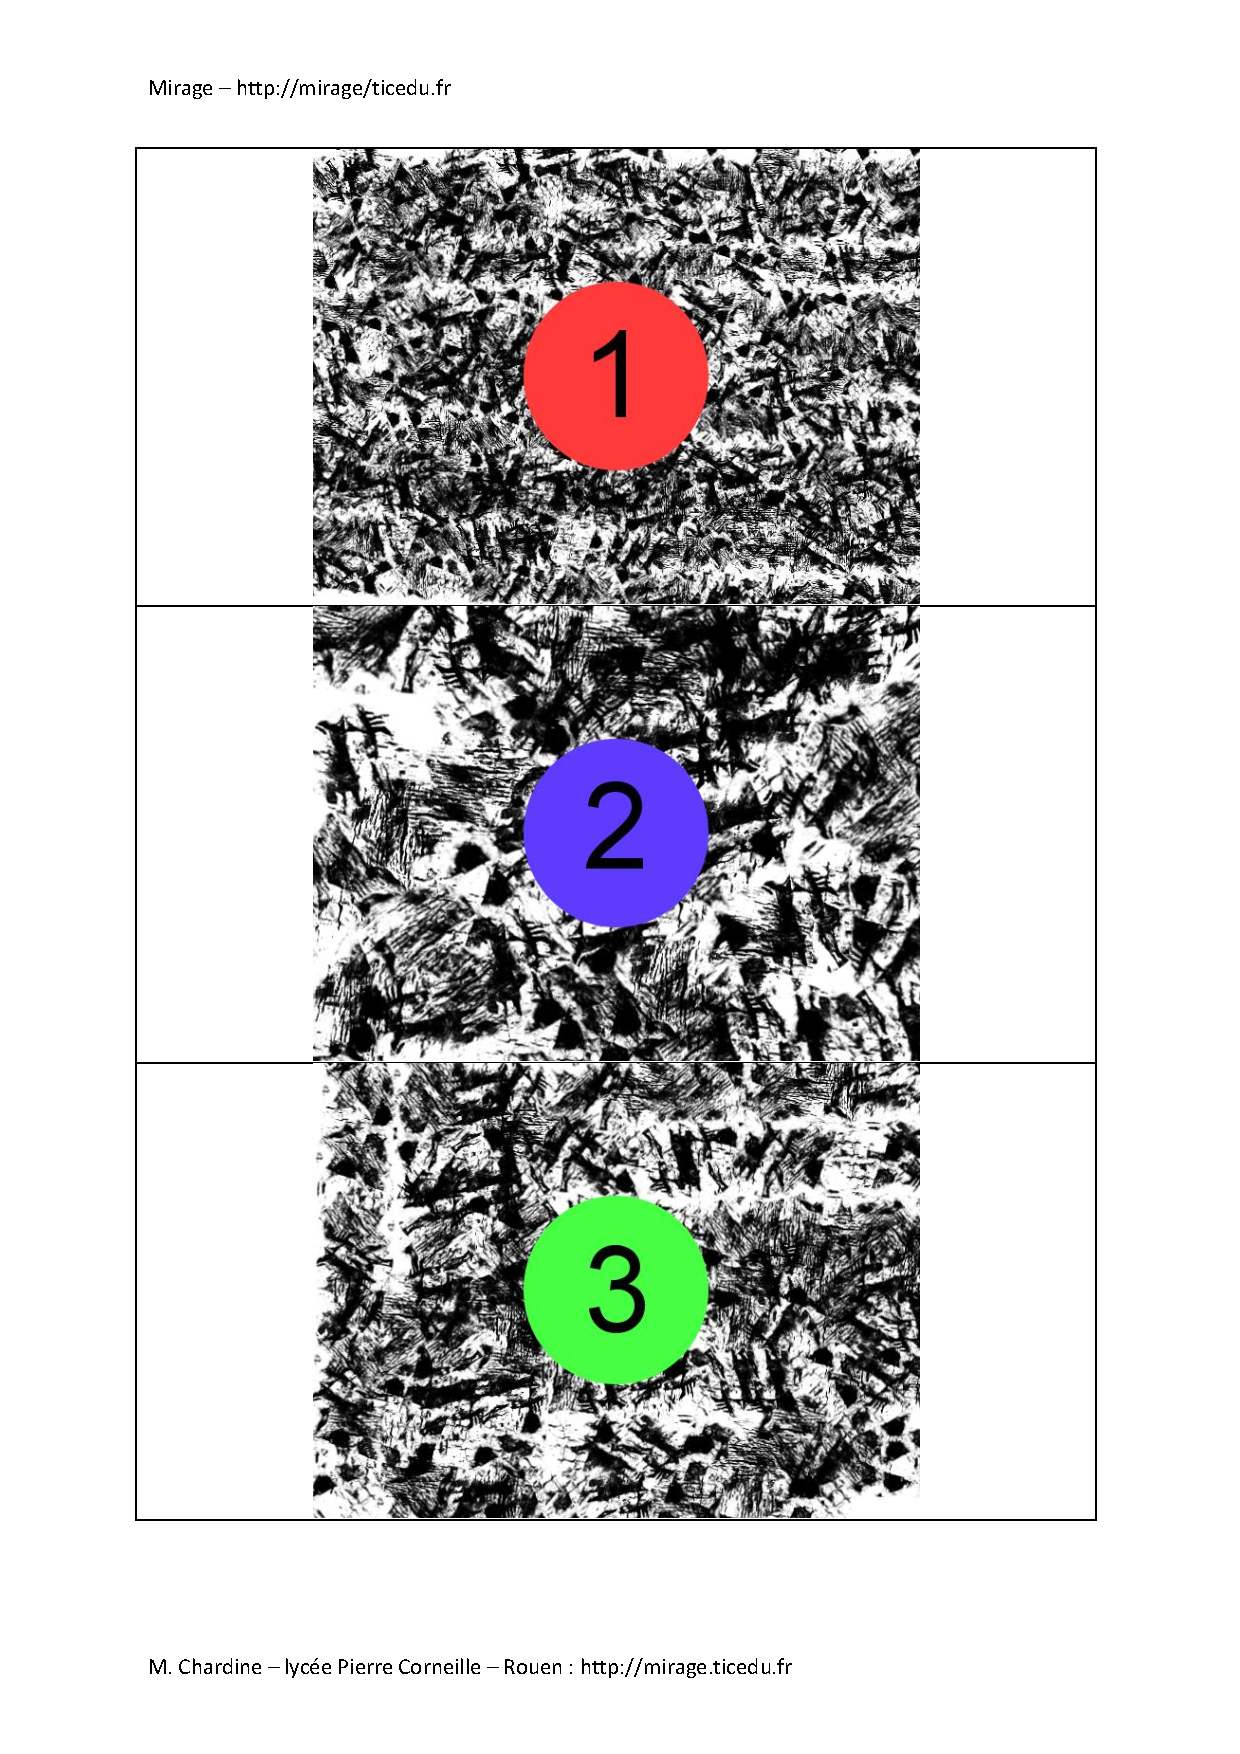
\includepdf[pages=1-4]{volume/marqueurs.pdf}

Et voilà la solution :
\begin{enumerate}
\item Cube $$ V= c^3$$
\item Pavé droit $$ V= l\cdot L \cdot h$$
\item Boule $$ V= \frac{4}{3}\pi r^3$$
\item Cylindre $$ V= \pi r^2 \cdot h$$
\item Cône $$ V= \frac{\pi r^2 \cdot h}{3}$$
\item Pyramide à base carrée $$ V= \frac{c^2 \cdot h}{3}$$
\item Pyramide à base triangle $$ V= \frac{\frac{b\cdot h'}{2}\cdot h}{3}$$
\item Prisme $$ V= b\cdot h' \cdot h$$
\item Prisme tronqué $$ V= \frac{B+b}{2} \cdot h' \cdot h$$
\item ? $$ V= \mbox{Aire de la base } \cdot h$$
\item ? $$ V= \mbox{Aire de la base } \cdot h$$
\item ? $$ V= \mbox{Aire de la base } \cdot h$$
\end{enumerate}

De manière générale, pour un prisme droit la formule est 
$$
\mbox{Aire de la base} \cdot \mbox{Hauteur}
$$

\section{Exercices}

\subsection{Calculs sur les aires}

\begin{exercice}
Chercher le périmètre d'un rectangle qui a pour dimensions : 7,30 m sur 2,60 m. 
\end{exercice}

\begin{exercice}
Chercher les côtés d'un rectangle sachant que le périmètre a 13 m et que la largeur est les ${}^{5}/{}_{8}$de la longueur.
\end{exercice}

\begin{exercice}
Un particulier a acheté un jardin carré à Fr. 2250.– l'are. Il l'a fait entourer d'une clôture qui coûte Fr. 5040.– à raison de Fr. 45.– le mètre. Combien a-t-il dû payer en tout ?
\end{exercice}

\begin{exercice}
La façade d’un monument est formée d’une partie rectangulaire de 15 m de longueur surmontée d’un fronton triangulaire de 3,50 m de hauteur. La surface de la façade est de 83,75 m2 .
Quelle est la surface de la partie rectangulaire ?
\begin{center}
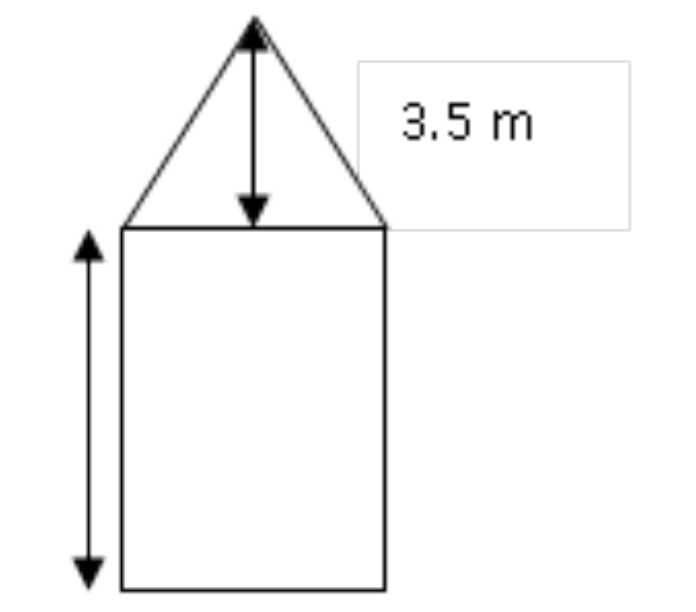
\includegraphics[width= 0.4\textwidth]{volume/image/ex4.png}
\end{center}
\end{exercice}

\begin{exercice}
Un champ a la forme d’un trapèze rectangle dont les bases mesurent 120 m et 80 m et  la hauteur 60 m. Il est traversé par une route de 10 m de large selon la figure ci-dessous. Calculer la surface de chacune des surfaces cultivables.
\begin{center}
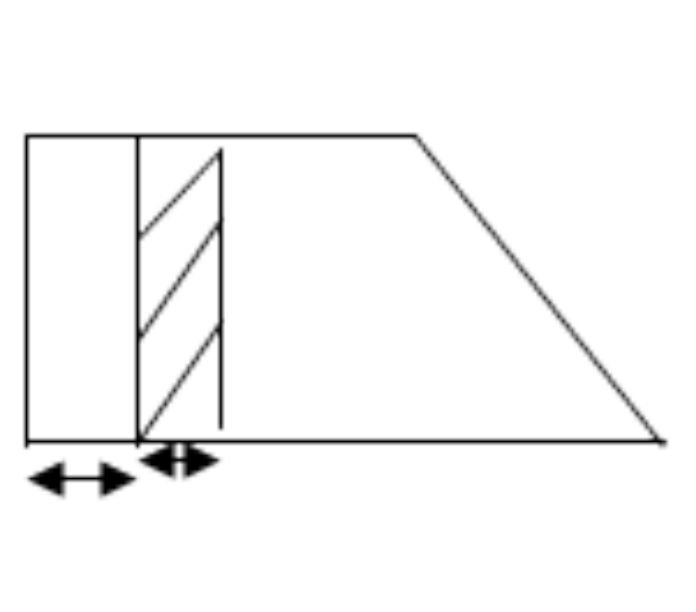
\includegraphics[width= 0.4\textwidth]{volume/image/ex5.png}
\end{center}
\end{exercice}

\begin{exercice}
Sur une carte à l’échelle \[1:2000\], une parcelle de terrain à la forme d’un trapèze dont les bases ont 12,5 cm et 9 cm et la hauteur 6 cm. On l’échange contre un terrain rectangulaire de même surface ayant 200 m de longueur. 
Calculer la largeur du rectangle et le prix de la clôture qui l’entoure à Fr. 50.– le mètre.
\end{exercice}

\begin{exercice}
Un coffret mesure 30 cm de long, 20 cm de large et 12 cm de hauteur. Pour le recouvrir sur toutes ses faces, sauf le fond, on dispose d’une glace de 0,80 m de long sur 0,40 m de large. 
Quelle est la surface de la glace inutilisée ?
\end{exercice}

\begin{exercice}
A la terrasse d’un café, il y a 6 caisses à fleurs, dont les parois sont peintes en vert. Chaque caisse mesure : 1 m de long, 0,40 m de large et 0,50 m de haut. 
S’il faut 200 g de peinture par m2, calculer la dépense, la peinture valant Fr. 4.– le kg.
\end{exercice}

\begin{exercice}
Une salle de classe a 7,80 m de long, 5,50 m de large et 4,20 m de haut. On recouvre les murs et le plafond de deux couches de peinture à Fr. 15.— le kg. 
Sachant qu’il faut 350 g de peinture par m2, quelle sera la dépense ? 
On déduira 2 fenêtres de 2,50 m sur 2,80 m chacune et une porte de 2,70 m sur 0,80 m.
\end{exercice}

\begin{exercice}
Sur une table ronde de 1,20 m de diamètre, on peint une bordure large de 6 cm. 
Quelle est la surface de la bordure ?
\end{exercice}

\begin{exercice}
Un bassin circulaire est entouré d’un terrain large uniformément de 7 m qu’on désire ensemencer en gazon. 
Quelle quantité de graines, à raison de 50 g par m2, doit-on acheter, sachant que le bord extérieur de la pelouse mesure 77 m ?
\end{exercice}

\begin{exercice}
Une piscine de forme rectangulaire de 56 m de long et de 24 m de large est terminée à ses extrémités par deux demi-cercles. On veut établir tout autour un trottoir bétonné de 2,7 m qui revient à Fr. 9,50 le m2. 
Quelle dépense fait-on ? 
\end{exercice}

\begin{exercice}
La grande circonférence d'une couronne mesure 18,8495559 m. Les rayons ont une différence de 1 m. 
Quelle est la surface d'un secteur de cette couronne ayant $70^\circ$ ($\pi =3.14$) ?
\begin{center}
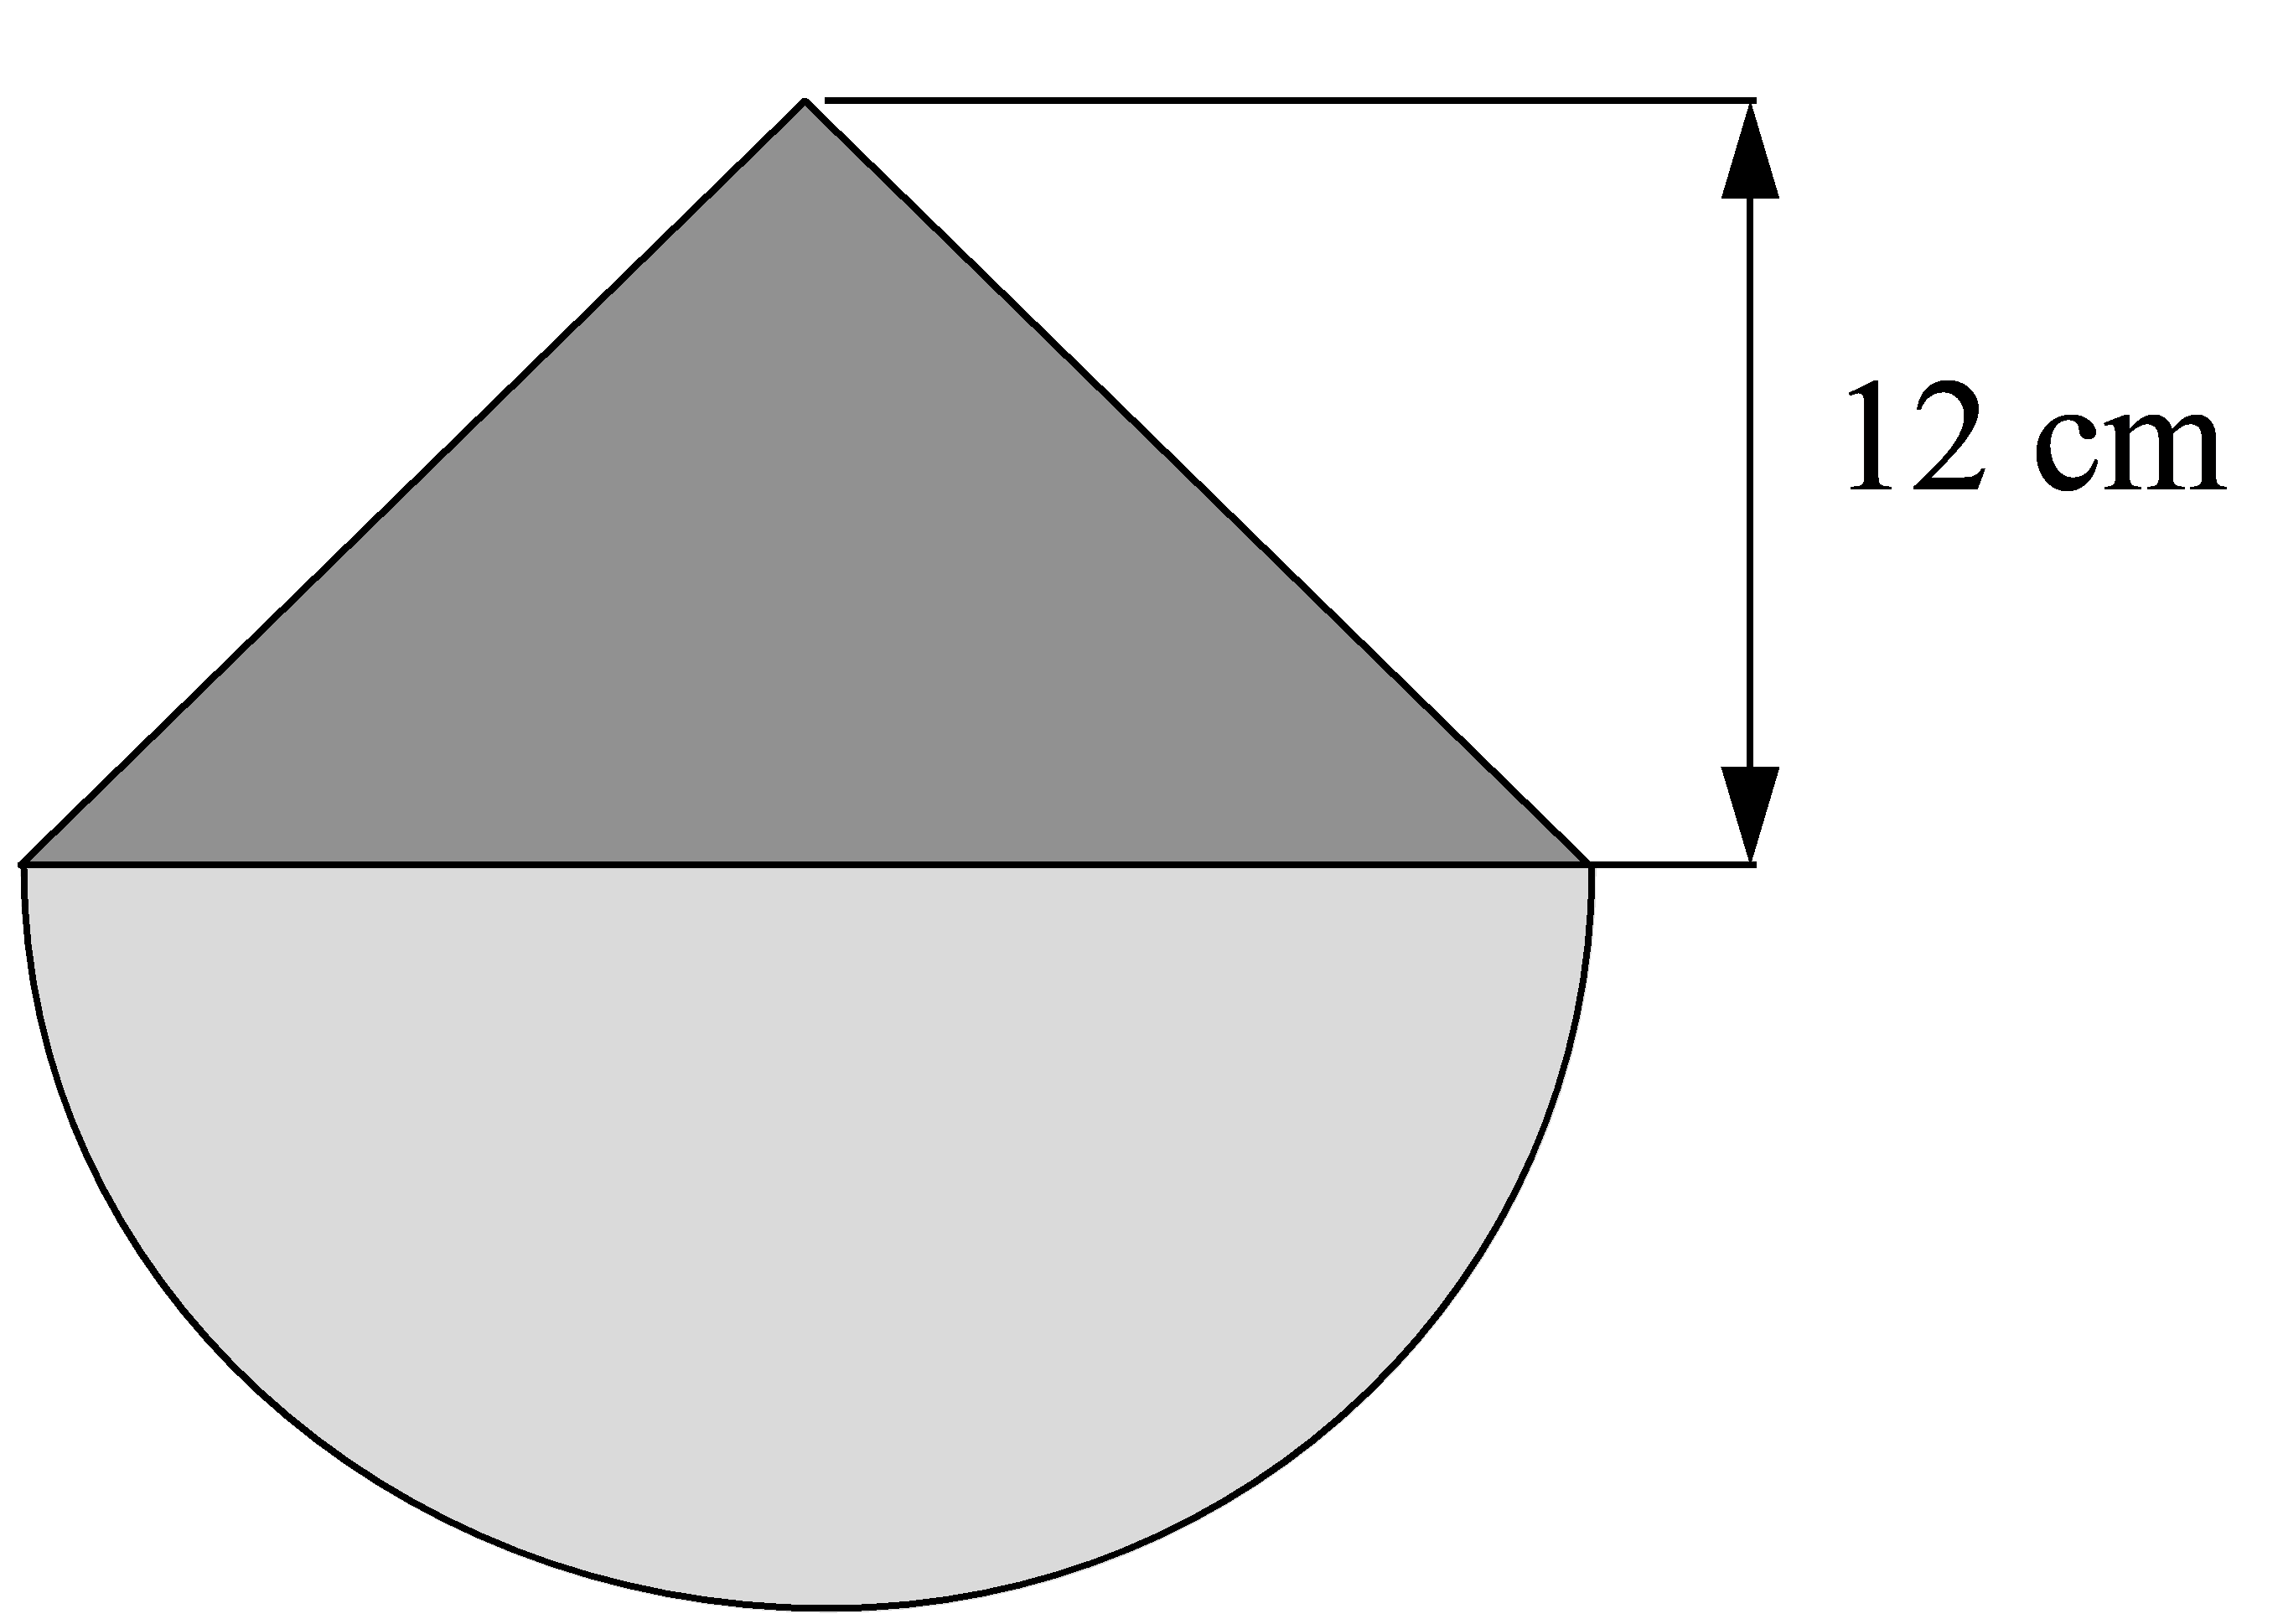
\includegraphics[width= 0.4\textwidth]{volume/image/ex13.png}
\end{center}
\end{exercice}

\begin{exercice}
Sachant que la surface du triangle est de 192 cm2 , calculer la surface totale de cette pièce. 
\end{exercice}

\begin{exercice}
La roue d’une voiture fait 400 tours à la minute. La vitesse restant toujours la même, combien de kilomètres cette voiture parcourt-elle en 1 heure 25 minutes sachant que le diamètre de la roue est de 63 cm ? 
\end{exercice}

\begin{exercice}
Dans un bouquin de géométrie de 1901, à l’usage des écoles primaires de l’époque, on trouvait les problèmes suivants :
\begin{center}
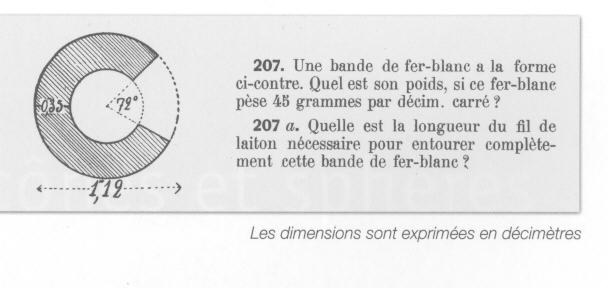
\includegraphics[width= 0.4\textwidth]{volume/image/ex17.png}
\end{center}
\end{exercice}

\subsection{Calculs sur les volumes}

\begin{exercice}
Quel est le volume d’un cône de 6 m de diamètre et de 7,10 m de hauteur ?
\end{exercice}

\begin{exercice}
Un presse-papier en marbre a la forme d’une pyramide dont la base est un carré de 24 cm de pourtour et dont la hauteur est de 4,5 cm . Quel est le poids de ce presse-papier, si le dm3 pèse 2,7 kg.
\end{exercice}

\begin{exercice}
La plus grande pyramide d’Egypte, dont la hauteur mesure 142 m a pour base un carré de 233 m de côté. La pyramide supposée pleine, quelle serait la longueur d’un mur de 2 m de haut et 50 cm de large construit avec les pierres de cette pyramide ?
\end{exercice}

\begin{exercice}
Calculer le volume de cette borne. 
\begin{center}
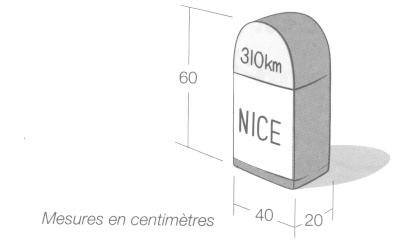
\includegraphics[width= 0.4\textwidth]{volume/image/volume4.png}
\end{center}
\end{exercice}

\begin{exercice}
Quelle est la hauteur d’un cône de 77 dm3 de volume et 84 cm de diamètre ? 
\end{exercice}

\begin{exercice}
Un cube a 36 cm d’arête. Combien de cubes de 18 mm d’arête faut-il pour le remplir exactement ?
\end{exercice}

\begin{exercice}
Un tas de briques a la forme d’un cube de 1,20 m d’arête et contient 1512 briques. Combien de briques semblables y a-t-il dans un autre tas cubique de 6 m de côté et quel est leur prix à raison de Fr. 140.— le mille ?
\end{exercice}

\begin{exercice}
Une cour a la forme d’un trapèze dont les bases mesurent 47 m et 43 m, et la hauteur 30 m. On étend sur cette cour 81 tombereaux de terre contenant chacun 0,9 m3. Quelle sera l’épaisseur moyenne de la couche de terre ?
\end{exercice}

\begin{exercice}
Une colonne, dont la base est un hexagone régulier, a un volume de 1245,6 dm3. Le côté de la base mesure 40 cm et l’apothème 34,6 cm. Quel est le prix de la peinture de cette colonne si l’on demande Fr. 21.— par m2 ?
\end{exercice}

\begin{exercice}
La base d’un prisme droit est un losange de 15 cm de côté, 18 cm de petite diagonale et 24 cm de grande diagonale. Sachant que l’aire latérale de ce prisme est de 1920 cm2, calculer son volume.
\end{exercice}

\begin{exercice}
Calculer la masse de cette pièce en acier sachant que 1 cm3 d’acier pèse 
7,8 g. Cotes en cm.
\begin{center}
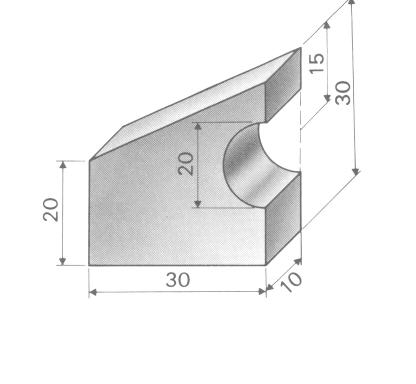
\includegraphics[width= 0.4\textwidth]{volume/image/volume11.png}
\end{center}
\end{exercice}

\begin{exercice}
Une portion de fromage a un volume de 27 cm3. Calculer l’angle $\alpha $ du secteur de base sachant que le rayon mesure 5,1 cm et que l’épaisseur de la portion est de 2 cm. 
\begin{center}
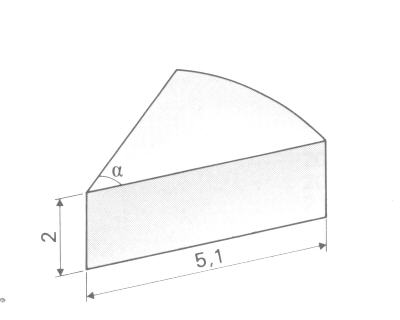
\includegraphics[width= 0.4\textwidth]{volume/image/volume12.png}
\end{center}
\end{exercice}

\begin{exercice}
Calculer la masse de cette pièce en aluminium sachant que la masse de 1 dm3 d’aluminium est 2,7 kg. 
\begin{center}
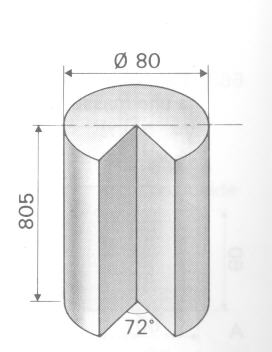
\includegraphics[width= 0.4\textwidth]{volume/image/volume13.png}
\end{center}
Cotes en cm. 
\end{exercice}

\begin{exercice}
Un ballon à air chaud a un rayon de 12 m. Quel volume d’air doit-on chauffer pour faire décoller ce ballon ? 
\begin{center}
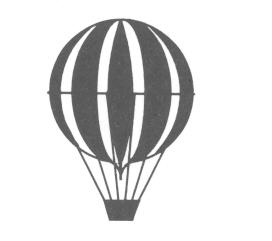
\includegraphics[width= 0.4\textwidth]{volume/image/volume14.png}
\end{center}
\end{exercice}

\begin{exercice}
Ce ballon de laboratoire est rempli à 1 cm de l’ouverture. Calculer sa contenance en dl, si le rayon du ballon mesure 11,5 cm, le diamètre du tube cylindrique 2 cm et sa hauteur 15 cm. 
\begin{center}
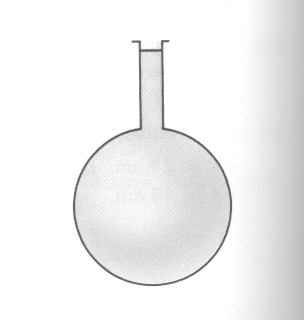
\includegraphics[width= 0.4\textwidth]{volume/image/volume15.png}
\end{center}
\end{exercice}